\documentclass{article}

\PassOptionsToPackage{numbers}{natbib}
\usepackage[final]{neurips_2023} % provided style file

\usepackage[utf8]{inputenc} % allow utf-8 input
\usepackage[T1]{fontenc}    % use 8-bit T1 fonts
\usepackage{hyperref}       % hyperlinks
\usepackage{url}            % simple URL typesetting
\usepackage{booktabs}       % professional-quality tables
\usepackage{amsfonts}       % blackboard math symbols
\usepackage{nicefrac}       % compact symbols for 1/2, etc.
\usepackage{microtype}      % microtypography

\usepackage{tabularx} % For tables with specified width
\usepackage{hyperref} % For hyperlinks
\usepackage{booktabs} % For better table lines
\usepackage{graphicx} % For including images
\usepackage{subcaption} % For subfigures

\usepackage{amsfonts}
\usepackage{amsmath}
\bibliographystyle{unsrtnat}
\usepackage{float}

\title{Predicting Cell Types in Non-Human Single Cell RNA Sequencing Data}

\author{
  Sean Connelly \\
  % examples of more authors
  \And
  Ryan Videgar-Laird \\
  \AND
  Stephanie Ting \\
}

\begin{document}

\maketitle

\section{Introduction}

The biology that underlies disease is heterogeneous, with multiple cell types and pathways within those cell types that contribute to the development of disease. All cells have DNA, the genetic code, that is transcribed into messenger RNA (mRNA), called gene expression. After these genes are expressed, the mRNA is then translated into proteins, which go on to perform different functions. mRNA can be expressed at different levels, depending on which proteins are needed by the given cell type. These different levels of mRNA expression can characterize cells and allow further analysis of their contribution to disease biology \cite{segundo-valIntroductionGeneExpression2016}.

The mRNA produced can be quantified at the cellular level, called single cell RNA sequencing (scRNAseq), to obtain a ‘fingerprint’ of different cell types and can be compared between normal or disease conditions to find how these cell types change. scRNAseq data is processed into a gene expression matrix, which has dimensions of $m$ cells x $n$ genes. After performing quality control steps, normalizing and scaling this gene expression matrix, this matrix undergoes dimensionality reduction to compress this dataset that contains many features (genes) to see how these cells relate to one another. The patterns of how cells vary compared to one another can be clustered using any algorithm of one’s choosing. The resulting clusters represent certain types of cells that may be characterized and classified \cite{aljanahiIntroductionAnalysisSingleCell2018}.

Classifying single cells has mainly focused on utilizing three categories of techniques. The first class of techniques annotate these clusters through comparing the differential expression (greater number of counts) of the genes in a given cluster with every other cluster through statistical tests, like the Wilcoxon rank sum test \cite{wilcoxonIndividualComparisonsGrouped1946}. These differentially abundant genes in each cluster can be compared to experimentally validated genes that characterize cell types to identify the label for that cluster. The second class of techniques correlates the newly generated dataset with a reference dataset to annotate cell clusters \cite{stuartComprehensiveIntegrationSingleCell2019}. This reference dataset can be other single cell RNA sequencing data or bulk RNA sequencing of specific cell types individually or over a time series. Lastly, the third class of techniques uses supervised learning, which utilizes previously generated data to train a model to classify cell types. Some examples of potential models to implement could be logistic regression, support vector machine or random forest, to name a few \cite{heumosBestPracticesSinglecell2023}.

Many of these tasks have been focused on human data, where there has been much focus on diseases that affect many people domestically, but not much focus on those that have broad impacts globally. One such disease is malaria, a parasitic infection that resulted in 247 million cases in 2021 and causes a large burden of morbidity and mortality globally \cite{organizationWorldMalariaReport2022}. Malaria has a complex life cycle, which starts in the mosquito vector to result in infection of a human host. When individuals are sick with malaria, the parasite replicates in the blood cells and causes these blood cells to lyse when the parasite replicates. These replication stages have unique gene expression patterns and single cell RNA sequencing provides a key benefit to further understand how these genes change per cell stage. These same concepts can be applied to other neglected diseases and hosts. We would like to build a powerful, simple and efficient model that can classify cell types on these sources of data. 

Previous works have used attention weights from transformer based models to identify biomarkers from cell type prediction \cite{chenTransformerOneStop2023} \cite{yangScBERTLargescalePretrained2022}. However, these methods rely on large amounts of training data and manually curated expert knowledge that are not available for organisms such as malaria. In our study we attempt to create a model with comparable accuracy that does not require either of these. Our approach is to use these methods as a foundation to build a simpler model that is less computationally expensive and works on non-human, non-mouse datasets. Our model will also not rely on manual curation of knowledge, which is often inconsistently annotated and formatted.

\subsection{Related Work}

Two previous studies have introduced methods that successfully use attention based models to predict cell type in scRNAseq. The first one, TOSICA, uses a three part approach of cell embedding, multi-head self attention, and then cell type classification \cite{chenTransformerOneStop2023}. TOSICA is highly accurate for both mouse and human data. This model, however, relies on curated expert knowledge in the cell embedding stage to provide pathway information critical to identifying cell types. The second model, scBERT, uses an adaptation of BERT, a natural language processing model on scRNAseq where the transformer architecture is replaced with a performer in order to better handle larger scale input data \cite{yangScBERTLargescalePretrained2022}. This model is trained with data from millions of cells from a variety of different biological contexts. scBERT not only predicts cell type with very high accuracy, it also has interpretability in that the prediction rediscovers known biomarker genes of each cell type. However, scBERT does require an immense amount of training data and has only been tested on human data. It is also a complex model that is computationally intensive.


\section{Methods}
\subsection{Data Processing}

Anndata \cite{virshupAnndataAnnotatedData2021} and Scanpy /cite{wolfSCANPYLargescaleSinglecell2018} were used to create efficient data objects and  follow best practices for scRNA-seq analysis. The datasets represented in Table 1 have to be accessed from their data repositories to obtain the $m$ x $n$ matrix. We implemented quality control filtering and normalization on these datasets through thresholding cells to only those with 200 or more expressed genes and filtering genes to those expressed in 3 cells or more. Counts were then normalized so that all cells had the same total count and log transformed (see https://scanpy.readthedocs.io/en/stable/generated/scanpy.pp.log1p.html). These quality control (QC) steps help reduce noise from experimental prep from sources, such as low quality cells and environmental contamination, and stabilize variance across cells \cite{heumosBestPracticesSinglecell2023}. The output is a gene expression matrix $X$, with dimensions $m$ cells by $n$ genes. We aimed to predict the different life stages of the malarial parasite (4 total classes: rings, early trophs, late trophs, and schizonts) and cell types reflected in the liver cancer cell atlas (7 total classes: B cells, CAFs, Malignant cells, T cells. TAMs, TECs, and unclassified).

Let \(y\) represent total gene counts for a given cell, and \(s_c\) represent the size factor for that cell. Counts are then shifted by:

\begin{displaymath}
% \label{eq:log_trans}
f(y) = log\left(\frac{y}{s_c} + y_0 \right)
\end{displaymath}

The size factor for a given cell designed to account for variation in cell size (larger cells typically contain more genetic transcripts) and sampling effects. Let \(L\) represent the median raw count depth across all cells. Then \(s_c\) is calculated across all genes, \(g\), per cell: 

\begin{displaymath}
% \label{eq:s_c}
s_c = \frac{\sum_g y_{gc}}{L}
\end{displaymath}

\subsection{Logistic Regression}

We first employed multinomial logistic regression, as implemented in the package scikit-learn \cite{pedregosaScikitlearnMachineLearning2011}. The model predicts probability $\hat{P}(y_i = k | x_i)$, out of $k$ different classes. The probabilities are determined using this softmax function:

$$
\hat{P}(y_i = k | x_i) = \frac{\exp(x_i W_k + W_{0,k})}{\sum_{l=0}^{K-1} \exp(x_i W_l + W_{0,l})}
$$
where $W$ is a matrix of coefficients with each row $w_k$ corresponds to class $k$ and $W_{0,k}$ is the bias term for class $k$. The gene expression vector for each cell is detonated by $x_i$

The optimization objective is to minimize the negative log-likelihood with an added $L_2$ regularization term to mitigate overfitting:
 
$$
\min_{W} -C \sum_{i=1}^{n} \sum_{k=0}^{K-1} [y_i = k] \log(\hat{P}(y_i = k | X_i)) + \frac{1}{2} \lambda ||W||_F^2
$$
 
The Iverson bracket $[P]$ evaluates to 1 if predicate $P$ is true and 0 otherwise. The regularization term $\frac{1}{2} \lambda ||W||_F^2$ is the $L_2$ norm of the weight matrix $W$, where $\lambda$ is the regularization strength, helping to control the complexity of the model by penalizing large weights.

\subsection{SVM}

For the training matrix $X_{train}$ and a vector of labels $y$, SVM funds $w$ and $b$ such that the prediction of sign($w^T x + b$) is correct for all $x$ in $X_{train}$. The hinge loss function is optimized by the following primal problem, as detailed in \cite{pedregosaScikitlearnMachineLearning2011}:

$$
\min_{w, b} \frac{1}{2} w^Tw + C \sum_{i=1}^{n} \max(0, 1 - y_i(w^T \phi(x_i) + b))
$$

where $w$ are the weights, $b$ is the bias, $C$ is the regularization parameter, $x_i$ is the $i$-th training example, $y_i$ is the label of the $i$-th training example, and $\phi$ is the identity function.

\subsection{GCN}

Graph Convolutional Networks (GCNs) are utilized to capture the dependencies between cells in the gene expression matrix by considering the graph structure. A GCN learns hidden layer representations that encode both local graph structure and features of nodes. The layer-wise propagation rule, described in detail in \cite{kipfSemiSupervisedClassificationGraph2017} and implement through the Spektral package \cite{grattarolaGraphNeuralNetworks2020}, is defined as:
 
$$
H^{(l+1)} = \sigma(\hat{D}^{-\frac{1}{2}} \hat{A} \hat{D}^{-\frac{1}{2}} H^{(l)} W^{(l)})
$$
 
where $H^{(l)}$ is the matrix of activations at the $l$-th layer, $\hat{A} = A + I$ is the adjacency matrix of the graph with added self-connections, $\hat{D}$ is the degree matrix of $\hat{A}$, $W^{(l)}$ is a layer-specific trainable weight matrix, and $\sigma(\cdot)$ is a non-linear activation function ReLU. The input to the GCN model consists of a gene expression matrix X, which is $(m, n)$ and a weighted adjacency matrix with shape $(m, m)$, generated from computing a neighborhood graph of cells with the function scanpy.pp.neighbors. The model is trained in a 70% train and 30% test split. The output of the GCN is a set of softmax predictions with shape $(m, k)$, which correspond to the classification of cell types.


\subsection{Transformer}

Our goal for each model was to utilize the performer and transformer architecture with a novel embedding that did not rely on expertly curated knowledge. The gene expression for each cell was embedded through multiplying the gene expression matrix with $d_{model}l$ (performer: 128,transformer: 48)-dimensional embedding, consisting of learnable and randomly initialized embeddings with the counts per each gene concatenated to the end of each embedding to reach the total amount of layers in each embedding. The positional encoding for each gene was not needed, as gene expression is coordinated in cellular programs but not ordered in a given cell.

With our unique embedding, we split each embedding into 70% and 30% train-test splits. We used a batch size of 8 and up to 50 epochs. We used a stack of 2 identical transformer encoder layers \cite{vaswaniAttentionAllYou2023}. Each layer has two-head self attention and a fully-connected 200 hidden layer feed-forward network. Scaled dot-product attention is implemented through the dot production of query matrix $Q$ and key matrix $K$. These are divided by $\sqrt{d_{model}}$. Then a softmax function is applied to then obtain the attention weights on the values in matrix $V$:
$$
Attention(Q,K,V) = softmax(\frac{QK^T}{\sqrt{d_{model}}})V
$$
Multi-head attention is implemented as below:
$$
MultiHead(Q,K,V) = Concat(head_1,...,head_h)W^O
$$
where $head_i = Attention(QW_i^Q,KW_i^K,VW_i^V)$, $W_i^Q \in \mathbb{R}^{d_{model} \times d_k}$, $W_i^K \in \mathbb{R}^{d_{model} \times d_k}$, $W_i^V \in \mathbb{R}^{d_{model} \times d_v}$, $W^O \in \mathbb{R}^{hd_v \times d_{model}}$.

The fully-connected feed-forward network consists of a linear transformation, a ReLU activation, and another linear transformation:
$$
FFN(x) = max(0,xW_1 + b_1)W_2 + b_2
$$
where $W_1 \in \mathbb{R}^{d_{model} \times d_{ff}}$, $b_1 \in \mathbb{R}^{d_{ff}}$, $W_2 \in \mathbb{R}^{d_{ff} \times d_{model}}$, $b_2 \in \mathbb{R}^{d_{model}}$. The input and output have dimension $d_{model}$ dimension of the hidden layer $d_{ff}$ is set to 200. All sub-layers in the model output a $d_model$ dimensional output. We used cross entropy loss as our loss function. We average the output across these transformer encoder layers and use a linear classification layer to generate a $(m,k)$ matrix of classification predictions. 

\subsection{Performer}

The performer architecture \cite{choromanskiRethinkingAttentionPerformers2022} approximates full-rank attention through Fast Attention Via positive Orthogonal Random features (FAVOR+). The attention matrix $A$ is approximated using the form:
$$
A(i,j) = K(q_i^T, k_j^T)
$$
with $q_i$ and $k_j$ being the query and key row vectors, respectively. The kernel $K$ is approximated using the following expectation:
$$
K(x,y) = \mathbb{E}\left[ \phi(x)^T \phi(y) \right]
$$
where $\phi$ is the random feature map. For the lower rank randomized matrices $Q’$ and $K’$, with rows $\phi(q_i^T)^T$ and $\phi(k_i^T)^T$, respectively, the approximation is:
$$
\text{Att}_{\phi}(Q, K, V) = D^{-1}(Q'(\mathbb{K}')^T)V), \quad D = \text{diag}(Q'(\mathbb{K}')^T1_l)
$$
For the lower rank randomized matrices $Q’$ and $K’$, with rows $\phi(q_i^T)^T$ and $\phi(k_i^T)^T$, respectively, the fast attention approximation is:
$\widehat{Att_{\leftrightarrow}}(Q, K, V) = \hat{D}^{-1}(Q'((\hat{K}')^T V)), \quad \hat{D} = \text{diag}(Q'((\hat{K}')^T \mathbf{1}_L))$

Lastly for the Orthogonal Random features portion, the random feature map $\phi$ for functions $f1, \dots, f_l$, function $h(x)$ and the deterministic vectors $w_1, \dots, w_m$ $\sim^{iid}$ $D$ for some distribution is defined below:
$$
\phi(x) = \frac{h(x)}{\sqrt{m}} \left[ f_1(w_1^T x), \dots, f_1(w_m^T x), \dots, f_l(w_1^T x), \dots, f_l(w_m^T x) \right]
$$

For performer, $d_{model} = 64$ and 50 epochs, but dimensions of performer for the other layers are the same as the transformer model. As above, 4 layers for the performer encoder are used. Each layer has two-head self-attention and a 4 layer fully connected feed forward network. The output is averaged across performer encoder layers and input into a linear classifier to result in a $(m,k)$ matrix of classification predictions.

\subsection{Performance Metrics}

We evaluated the performance of the models through the F1 score, averaged per each class for each model:

$$
F1 = 2 \cdot \frac{\text{precision} \cdot \text{recall}}{\text{precision} + \text{recall}}
$$
where precision is defined as $TP/(TP + FP)$ and recall is defined as $TP/(TP + FN)$

\section{Results}

\subsection{Traditional Methods}

We began with two scRNAseq dataset (P. falciparum) from the Malaria Cell Atlas \cite{howickMalariaCellAtlas2019} and data from the liver cancer cell atlas \cite{maSinglecellAtlasTumor2021} to test out different supervised classification models. We began with these two datasets to compare a small non-human parasite dataset with a large human data, which we anticipated would perform well, as it has many cells and genes for each class. In addition, standard methods have been shown to perform well on this dataset \cite{shuklaSupervisedLearningPlasmodium2023} so it serves as a good baseline for later comparisons. 

Principal Component Analysis was performed to visualize how the given cells vary compared to one another. The cells are well stratified by developmental stage (Figure 1). To test the performance of two classic models for classification tasks, we used logistic regression (LR) and support vector machines (SVM), implemented through Scikit-learn \cite{pedregosaScikitlearnMachineLearning2011}. To incorporate more graph based information in our model, we used an implementation of a graph convolutional network in the Spektral package \cite{grattarolaGraphNeuralNetworks2020}, based on the work of Kipf and Welling \cite{kipfSemiSupervisedClassificationGraph2017}. The data was split into a 70\% training and 30\% test split. The input to the model was the filtered and normalized gene expression matrix along with the cell type labels.

For each model, we labeled the cells in the PCA as correct (blue) or incorrect (orange). Incorrectly predicted cells were spread throughout the PCA and did not concentrate within a certain cell type across all models (Figure 2). 

\begin{figure}[H]
	\centering
  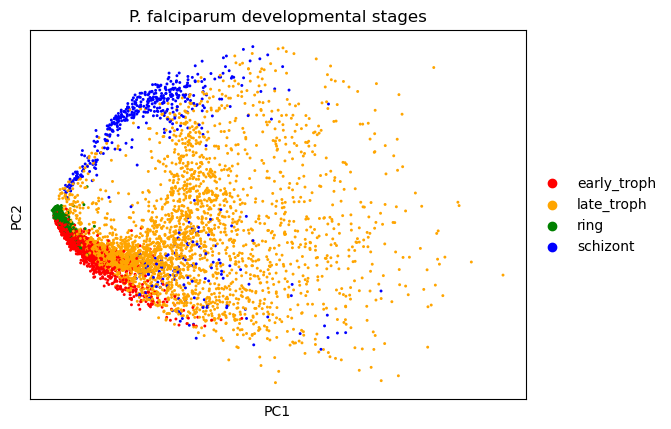
\includegraphics[width=0.8\textwidth]{figures/pca_Pf.png}
  \caption{Principal components analysis of \textit{P. falciparum} single cell RNA sequencing data, colored by lifecycle stage.}
  \label{fig:pfal_pca_true}
\end{figure}

\begin{figure}[!h]
  \centering
  \begin{subfigure}[b]{0.3\textwidth}
      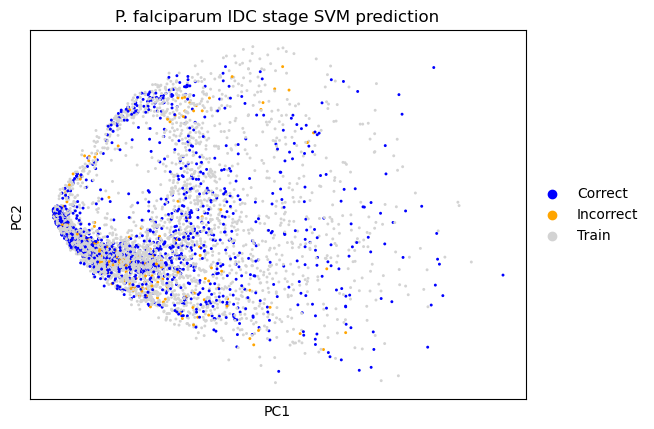
\includegraphics[width=\textwidth]{figures/pca_Pf_prediction_SVM.png}
      \caption{PCA of predictions from SVM model.}
      % \label{fig:sub1}
  \end{subfigure}
  \hfill
  \begin{subfigure}[b]{0.3\textwidth}
      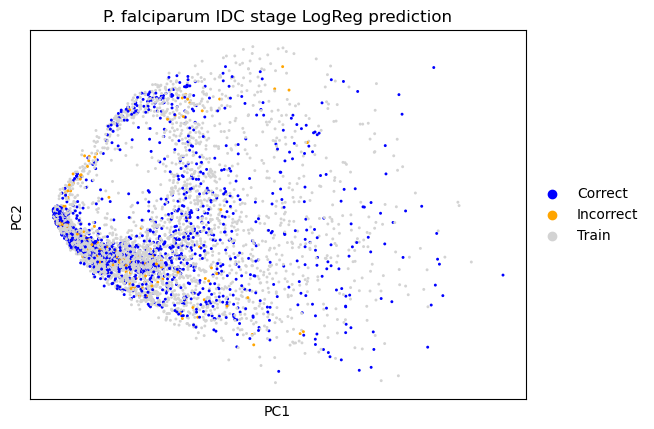
\includegraphics[width=\textwidth]{figures/pca_Pf_prediction_LogReg.png}
      \caption{PCA of predictions from logistic regression model.}
      % \label{fig:sub2}
  \end{subfigure}
  \hfill
  \begin{subfigure}[b]{0.3\textwidth}
      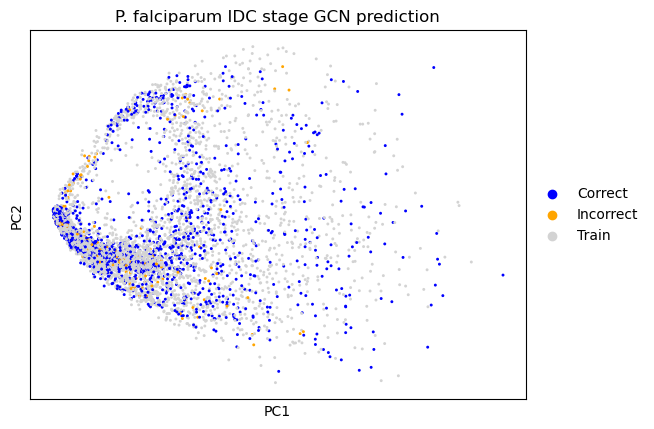
\includegraphics[width=\textwidth]{figures/pca_Pf_prediction_GCN.png}
      \caption{PCA of predictions from graph convolutional network model.}
      % \label{fig:sub3}
  \end{subfigure}
  
  \caption{Model performance visualized on PCA plots.}
  \label{fig:pfal_pca_pred}
\end{figure}

\subsection{Transformer Models}

<Talk about perforance of them>

We computed the F-1 score across all methods. Each model achieved F1 scores above 0.80 across at least two cell types. The transformer model is an expection <talk about high training loss variance, might need to adjust learning rate>(Figure \ref{fig:pfal_pred_f1}).

\begin{figure}[H]
  \centering
  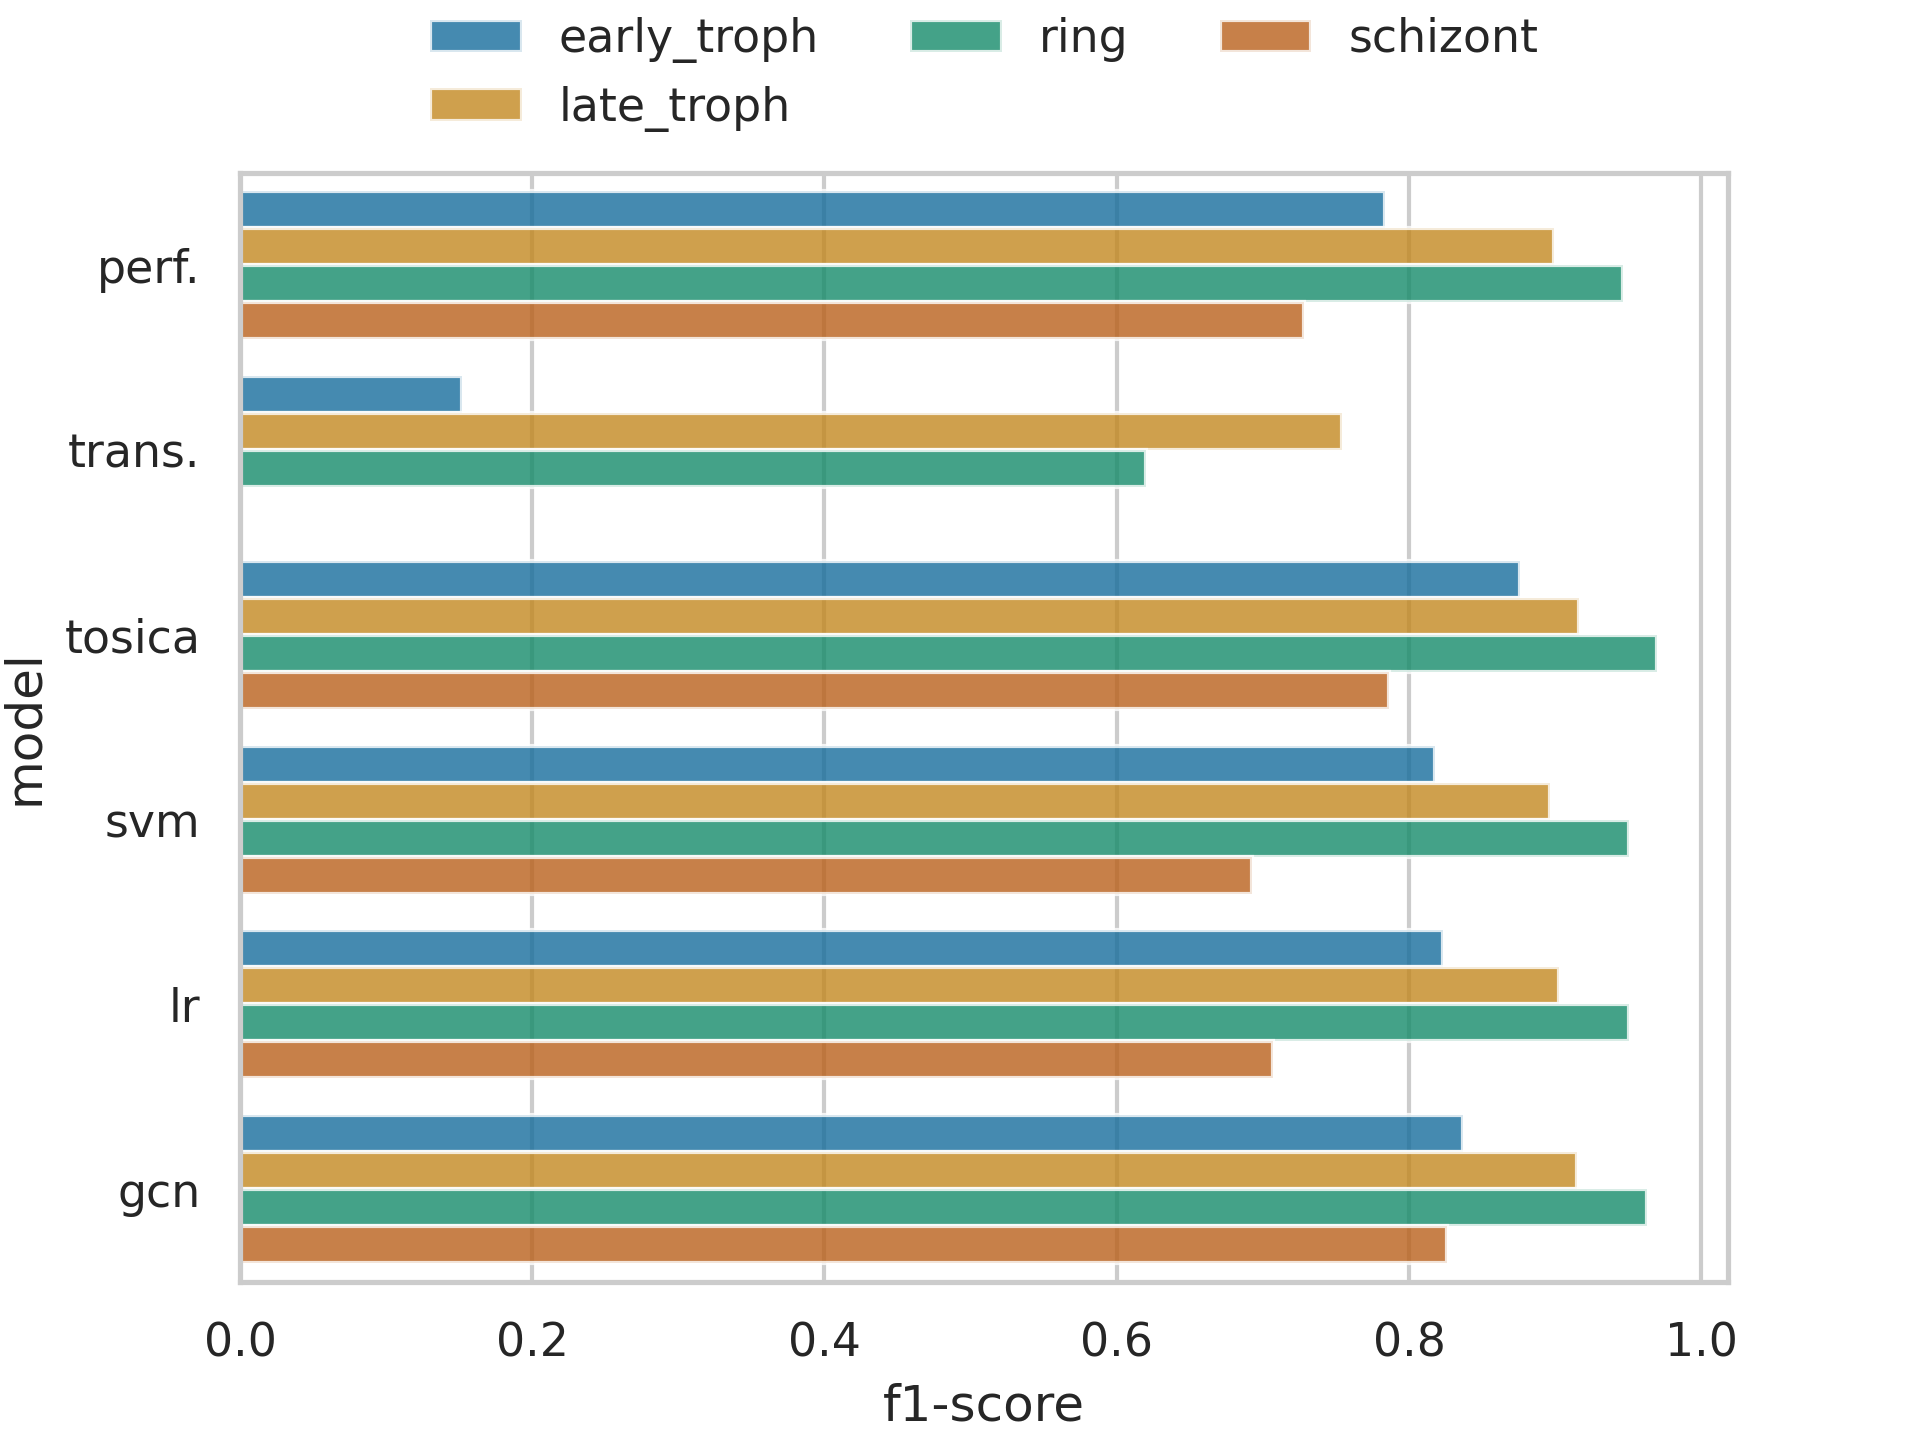
\includegraphics[width=0.8\textwidth]{figures/f1_scores_bar.png}
  \caption{Prediction accuracy of models on \textit{P. falciparum} single cell RNA sequencing data.}
	\label{fig:pfal_pred_f1}
\end{figure}



\begin{figure}[!h]
  \centering
  \begin{subfigure}[b]{0.4\textwidth}
      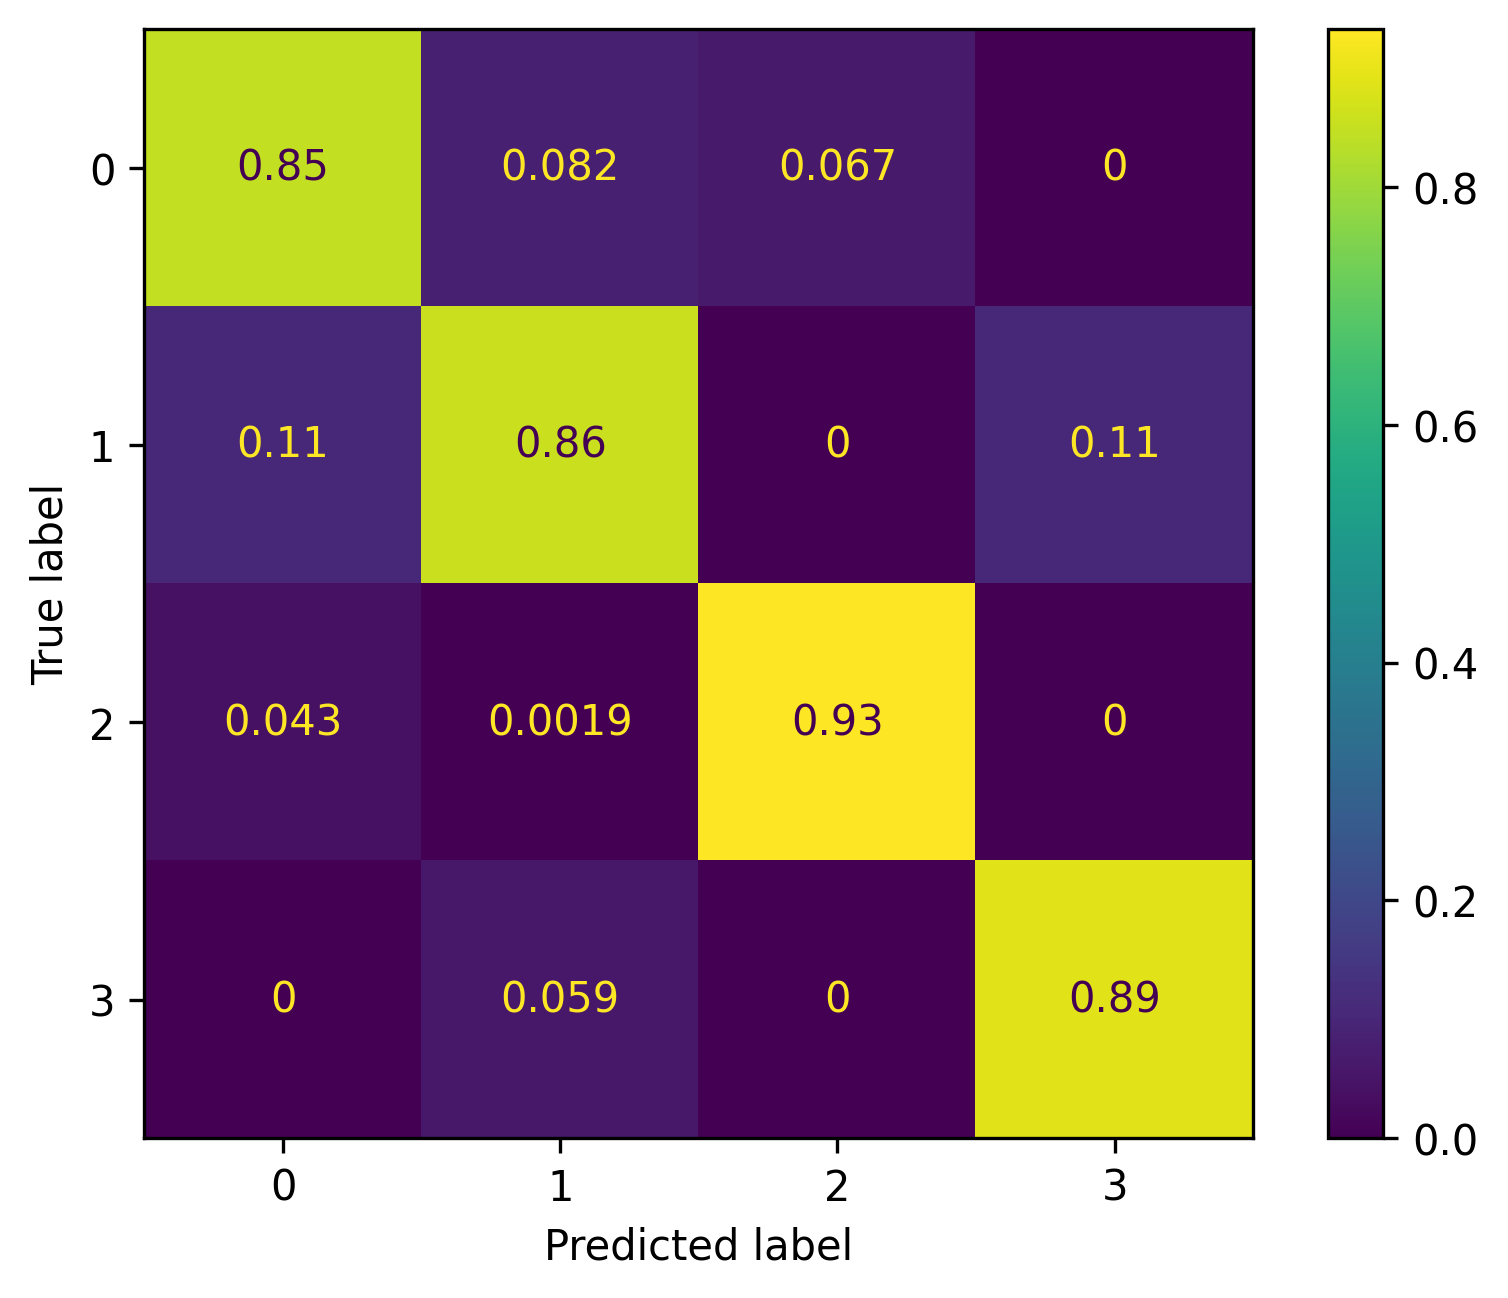
\includegraphics[width=\textwidth]{figures/performer_confusion.png}
      \caption{PerformerClassifier}
      % \label{fig:sub1}
  \end{subfigure}
  \hfill
  \begin{subfigure}[b]{0.4\textwidth}
      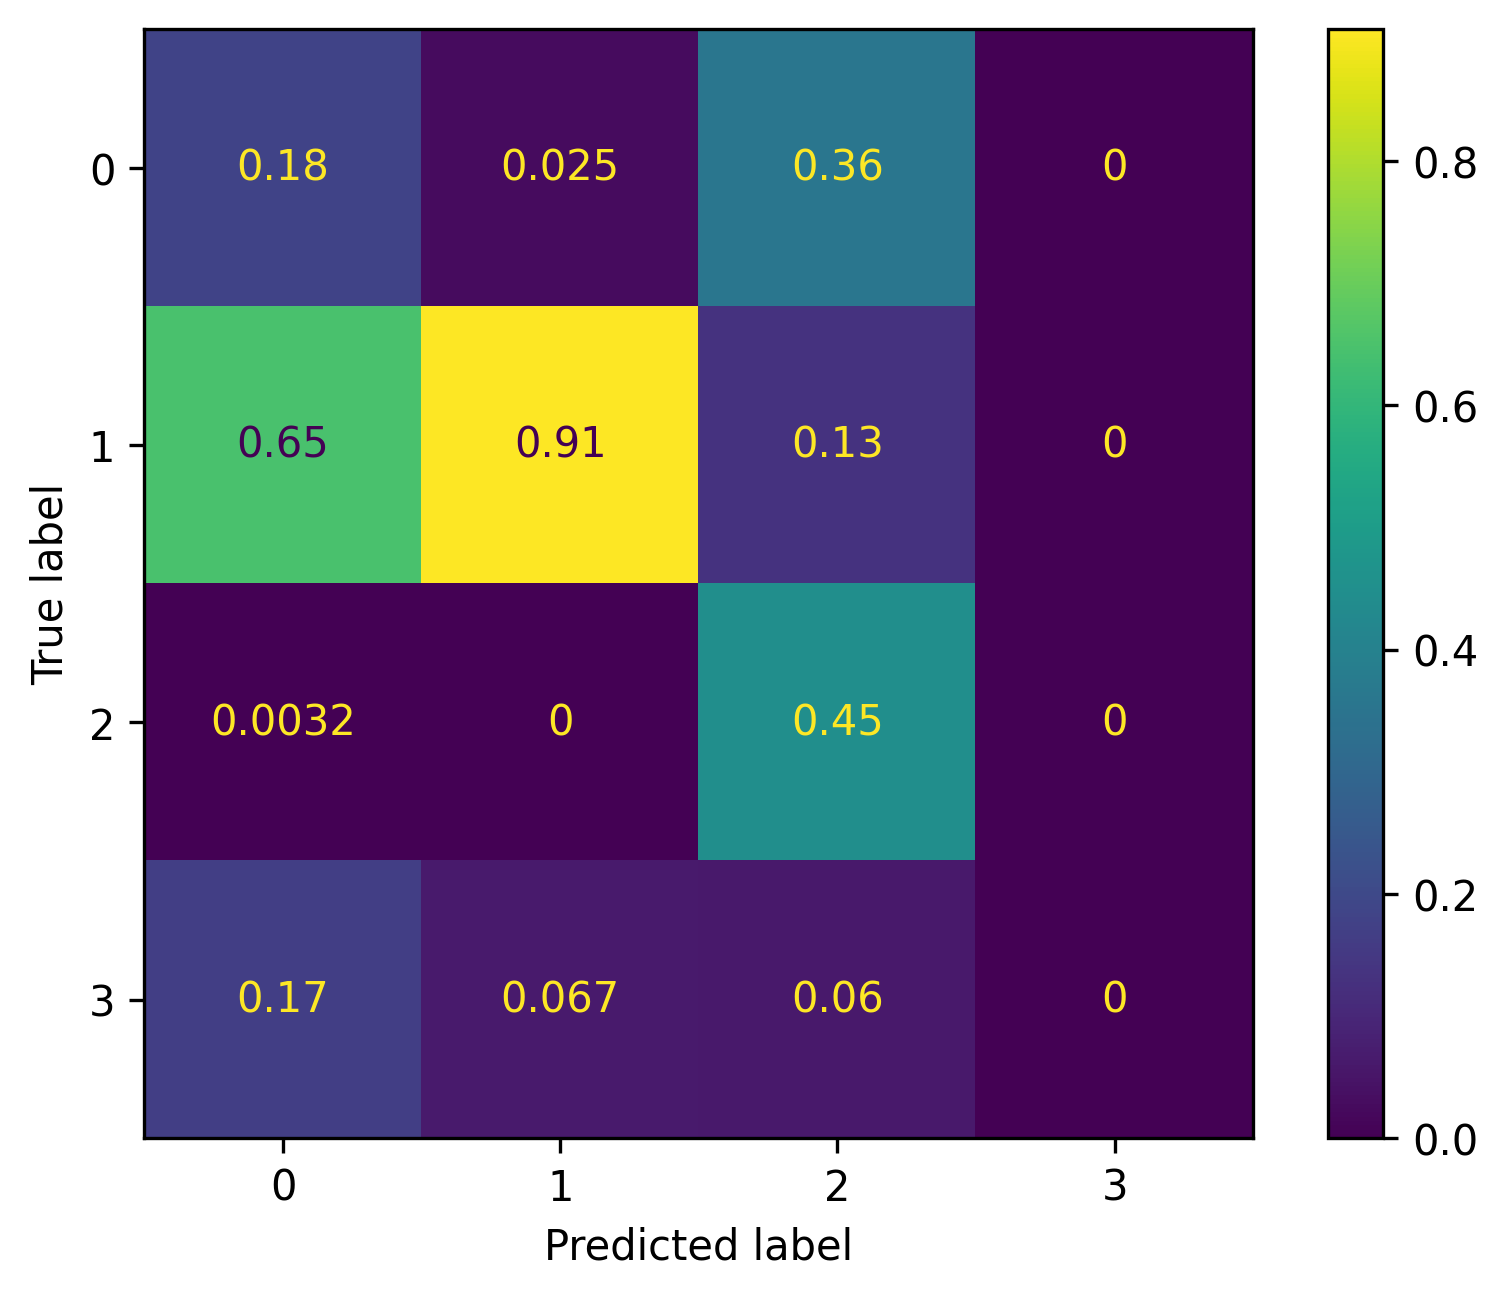
\includegraphics[width=\textwidth]{figures/transformer_confusion.png}
      \caption{TransformerClassifier}
      % \label{fig:sub2}
  \end{subfigure}
  \caption{Confusion matrices comparing our Performer and Transformer based classifiers in \textit{P. falciparum}. Classes 0-3 represent: early troph.; late troph.; ring; and schizont stages, respectively}
  \label{fig:pfal_confus}
\end{figure}


\subsection{Datasets}

We collated a list of scRNAseq datasets, which represent non-human, non-mouse datasets from a wide array of organisms and reference human and mouse datasets (Table \ref{tab:dat_summary}). The organisms include malaria, parasitic worm \emph{Schistosoma mansoni}, the cause of African sleeping sickness \emph{Trypanosoma brucei}, tick borne parasite \emph{Babesia microti}, zebrafish, and non-human primates. Through training and testing our model on a variety of organisms, we hope to create a model that transcends the need for manual knowledge and can find biomarkers of different cell types to better characterize these diseases. 

\begin{table}[!h]
  \caption{Summary of datasets that will be used in this study.}
  \label{tab:dat_summary}
  \centering
  \begin{tabularx}{\textwidth}{lXll}
    \toprule
    \textbf{Host} & \textbf{Source} & \textbf{Reference} & \textbf{Cells} \\
    \midrule
    Parasite & \href{https://github.com/vhowick/MalariaCellAtlas/tree/4e19a713d0681b118cc7e229133489f039b8766b/Expression_Matrices/10X/pf10xIDC}{GitHub} & \citet{howickMalariaCellAtlas2019} & 6,737 \\
    \midrule
    Human & \href{https://www.ncbi.nlm.nih.gov/geo/query/acc.cgi?acc=GSE151530}{GEO: GSE151530} & \citet{maMultiregionalSinglecellDissection2022} & 56,721 \\
    \bottomrule
  \end{tabularx}
\end{table}

\section{Conclusion}

Biomarker discovery is an inherently difficult procedure. An ideal biomarker is: generalizable across disease state and patient demographics; easy to measure (e.g. a simple blood draw); robust; and based upon a strong biological foundation related to the underlying disease etiology. Identification typically occurs through an iterative process of hypothesis generation followed by costly experimental validation. The procedure is often more akin to the ‘art’ of gambling, rather than science. Biology is immensely complex. Most potential biomarkers identified through computational methods quickly fall apart once interrogated in the lab. Additionally, there is a general feeling much of the low-hanging fruit (e.g. BRCA1/2 in breast cancer) has already been plucked. Therefore optimistic researchers frequently hope for new methods that better handle biological intrices and afford more precision. 

Naturally, this has led many to explore the use of transformer-based models due to their massive success in generative AI. To help address the utility of such models in genomic biomarker discovery, your authors skeptically jumped on the (perhaps already fading) transformer and attention bandwagon. We were motivated by the broad observation that biological models being published, such as scBERT or TOSICA, seem to miss the overall point and context of their ideal use. In pursuit of raw predictive power, they tend to build overly complex models that rely on huge datasets and external priors, such as scBERT’s use of gene2vec \cite{duGene2vecDistributedRepresentation2019}. While performant, such models may miss the chance to generate novel encodings that could help better inform downstream hypothesis generation. They are also less applicable to smaller, often niche datasets, such as malaria, which do not have large amounts of training data available, nor do they have curated knowledge available for masking.

We successfully adapted two new transformer models for single-cell type label prediction. Our models have comparable accuracy to previous work without relying on extremely large training datasets or manually curated knowledge, which will be instrumental in analyzing single cell RNAseq data in less well-studied organisms. However, we remain skeptical, as these models took considerably more computational resources to achieve performance on par with ‘traditional’, and more directly interpretable, methods such as logistic regression.



\bibliography{final_report}

\end{document}